
%(BEGIN_QUESTION)
% Copyright 2006, Tony R. Kuphaldt, released under the Creative Commons Attribution License (v 1.0)
% This means you may do almost anything with this work of mine, so long as you give me proper credit

Calculate the weight of an iron rod (D = 490.68 pounds per cubic foot), 5 feet long and 2 inches in diameter, as it hangs inside an empty vessel:

$$\includegraphics[width=15.5cm]{i00275x01.eps}$$

Next, calculate the amount of weight indicated by the scale as the vessel fills with water until 3 feet of the rod is submerged.  Hint: the metal rod will be {\it displacing} a volume of water 3 feet in length and 2 inches in diameter.

$$\includegraphics[width=15.5cm]{i00275x02.eps}$$

Be sure to show all your mathematical work so that your instructor will be able to check the conceptual validity of your technique(s).  A good way to check to see if you're solving the problem correctly is to check that each and every one of your intermediate calculations (i.e. the results you get mid-way during the process to arrive at the final answer) has real physical meaning.  {\bf If you truly understand what you are doing, you will be able to identify the correct unit of measurement for every intermediate result and also be able to show where that number applies to the scenario at hand}.

\vskip 20pt \vbox{\hrule \hbox{\strut \vrule{} {\bf Suggestions for Socratic discussion} \vrule} \hrule}

\begin{itemize}
\item{} Demonstrate how to {\it estimate} numerical answers for this problem without using a calculator.
\item{} How would your weight calculations be affected if the rod were made of some material other than iron?
\item{} How would your weight calculations be affected if the iron rod were a larger diameter but identical length?
\item{} How would your weight calculations be affected if the liquid had a density different from water?
\end{itemize}

\underbar{file i00275}
%(END_QUESTION)





%(BEGIN_ANSWER)

Dry weight = 53.52 pounds

\vskip 10pt

Submerged (by 3 feet) weight = 49.44 pounds

%(END_ANSWER)





%(BEGIN_NOTES)

$F_{dry} = (490.68 \hbox{ lb/ft}^3) (5 \hbox{ ft}) \left( \pi \left( {1 \over 12} \hbox{ ft} \right)^2 \right) = 53.52 \hbox{ lb}$

\vskip 10pt

$F_{buoyant} = (62.428 \hbox{ lb/ft}^3) (3 \hbox{ ft}) \left( \pi \left( {1 \over 12} \hbox{ ft} \right)^2 \right) = 4.086 \hbox{ lb}$

\vskip 10pt

$F_{apparent} = F_{dry} - F_{buoyant} = 53.52 - 4.086 = 49.439 \hbox{ lb}$




\vfil \eject

\noindent
{\bf Prep Quiz:}

What will happen to the weight registered by the scale if salt is added to the water to make it denser?

$$\includegraphics[width=15.5cm]{i00275x02.eps}$$

\begin{itemize}
\item{} The amount of weight will increase
\vskip 5pt 
\item{} The amount of weight will decrease
\vskip 5pt 
\item{} The amount of weight will remain unchanged
\vskip 5pt 
\item{} The tank will explode, taking the scale out with it
\end{itemize}





\vfil \eject

\noindent
{\bf Prep Quiz:}

What will happen to the weight registered by the scale if the water is drained and then replaced with pure alcohol (filled to the exact same height of 3 feet)?

$$\includegraphics[width=15.5cm]{i00275x02.eps}$$

\begin{itemize}
\item{} The amount of weight will increase
\vskip 5pt 
\item{} The amount of weight will decrease
\vskip 5pt 
\item{} The amount of weight will remain unchanged
\vskip 5pt 
\item{} The tank will explode, taking the scale out with it
\end{itemize}





\vfil \eject

\noindent
{\bf Summary Quiz:}

Calculate the apparent weight of this displacer when it is fully submerged, assuming it weighs 53.5 pounds dry:

$$\includegraphics[width=15.5cm]{i00275x03.eps}$$

\begin{itemize}
\item{} 49.2 pounds
\vskip 5pt 
\item{} 26.3 pounds
\vskip 5pt 
\item{} 46.7 pounds
\vskip 5pt 
\item{} 53.5 pounds 
\vskip 5pt 
\item{} 49.4 pouuds
\vskip 5pt 
\item{} 81.7 pounds
\end{itemize}

%INDEX% Physics, static fluids: buoyancy

%(END_NOTES)


